\documentclass[12pt]{article}
\usepackage{amsmath}
\usepackage{geometry}
\usepackage{algorithm,float}
\usepackage[noend]{algpseudocode}
%\setlength\parindent{0pt}
\usepackage{graphicx}
\usepackage{caption}
\usepackage{setspace}
\usepackage[font={small,it}]{caption}
\usepackage{enumitem}
\usepackage{amssymb}
\usepackage[noend]{algpseudocode}
\usepackage{algorithm}
\usepackage{bm}
\usepackage{color}
\usepackage{epstopdf}
\usepackage{pdflscape, amsthm}
\usepackage{subcaption}
\usepackage{multirow}
\usepackage{apacite}

\newcommand{\bred}[1]{\textbf{\textcolor{red}{#1}}}
\newcommand{\bblue}[1]{\textbf{\textcolor{blue}{#1}}}

\DeclareMathOperator*{\argmin}{\arg\!\min}
\DeclareMathOperator*{\argmax}{\arg\!\max}
\newtheorem{theorem}{Theorem}
\newtheorem{condition}{Condition}
\newtheorem{assumption}{Assumption}

% Keywords command
\providecommand{\keywords}[1]
{
  \small	
  \textbf{\textit{Keywords---}} #1
}

\title{A Note on the Advantage of Context in Thompson Sampling}
\author{Michael Byrd and Ross Darrow}

% \linespread{1.5}
\begin{document}

\maketitle

\begin{abstract}
Personalization has become a focal point of modern revenue management. 
However, it is often the case that minimal data is available to appropriately 
make suggestions tailored to each customer.
This has led to many products making use of reinforcement learning based  
algorithms to explore sets of offerings to find the best suggestions to 
improve conversion and revenue.
Arguably the most popular of these algorithms are built on the foundation of 
the multi-arm bandit framework, which has shown great success across a variety 
of use cases. 
A general multi-arm bandit algorithm aims to tradeoff adaptively exploring 
available, but under observed, recommendations, with the current known best
offering. 
While much success has been achieved with these relatively understandable 
procedures, much of the airline industry is losing out on better personalized 
offers by ignoring the context of the transaction, as is the case in the 
traditional multi-arm bandit setup.
Here, we explore a popular exploration heuristic, Thompson sampling, and note
implementation details for multi-arm and contextual bandit variants.
While the contextual bandit requires greater computational and technical 
complexity to include contextual features in the decision process, we 
illustrate the value it brings by the improvement in overall expected 
\end{abstract}

\keywords{bandit algorithms, online learning, e-commerce}

\section{Introduction}

Real-time, model-driven insights become increasingly important for maintaining a
competitive edge in the marketplace.
Many upcoming applications of revenue management require or will be enhanced by 
real-time experimentation. 
Some examples:
\begin{enumerate}
\item \textbf{Ancillary pricing}. 
While common to initialize ancillary prices with customer surveys and conjoint 
analysis \cite{green2001thirty}, after initial prices are set it's often useful 
to do live experiments to further optimize the prices. 
Even well-designed experiments may not accurately capture the the true 
willingness-to-pay of an item, and, worse, can not adapt to changing behaviors 
over time without further studies. 
\item \textbf{Personalized offers}.  
Recently, under mild assumptions, it was estimated that profits could be improved 
over 10\% by using personalized pricing \cite{dube2019personalized}.  
For an introduction to offer management for airlines, see 
\cite{vinod2018approach}.
\item \textbf{Online shopping and booking}. 
Airlines and online travel agencies want to experiment with different display 
approaches to improve conversion. 
\end{enumerate}
 
Offline analysis, such as traditional A/B/n testing, has shown to be too slow to 
adapt to the current rapidly changing marketplace.
The main criticisms being that an A/B/n test is expected to run for a 
predetermined amount of time while also uniformly allocating traffic allocation
regardless of recently observed findings.
To address these problems, reinforcement learning algorithms have been introduced
to quickly learn toward an optimal solution in real-time. 
Many problems fall into the bandit paradigm, which balances between recommending
new offerings with the current known-best offering.
The most well-known of these approaches is the multi-arm bandit 
\cite{whittle1980multi}.
The travel industry has begun making extensive use of multi-arm bandit algorithms
to address many web-scale problems.

While the multi-arm bandit works well, the traditional algorithms ignore the
available contextual data.  
Incorporating each unique context into business decisions has been shown to help
adaptively address similar issues with minimal data.
For example, a well-known empirical experiment with the contextual bandit 
illustrated substantial gains in performance for personalizing news articles
\cite{li2010contextual}.
To illustrate the advantage of using context, we explore a multi-arm bandit 
algorithm employed by many in the travel industry, Thompson sampling, and
show how recent advancements extended it to handle context.

\subsection{Overview}

In Section \ref{sec:background} we present the foundation for bandit algorithms.
This includes reviewing Thompson sampling.  
Section \ref{sec:pgts} then further inspects a contextual bandit algorithm using 
Thompson sampling. 
Here, we review the algorithm and inspect improvements to ease computation.
In Section \ref{sec:simulation} we implement a simulation study to investigate 
the potential performance improvements for the contextual algorithm over bandit 
algorithms that ignore the context.
Finally Section \ref{sec:conclusion} offers final thoughts and future improvements.

\section{Background} \label{sec:background}

We consider the bandit problem with binary reward.
For time step $t = 1, 2, \ldots$ suppose a recommendation is to be made from one 
of $K$ possible options.
Upon being received, the recommendation is either selected or not selected; we 
note that these concepts can easily be adapted to incorporate the profitability
into the decision process.
The goal is to recommend the option that has the highest chance of success.
Suppose, of the $K$ options available to recommend, that each option has $p_A$ 
features.
We refer to each option as an \textit{arm}, where 
$\bm{a}_i \in \mathbb{R}^{p_A}$
denotes the set of features associated with arm $i$. 
Further suppose each instance has an additional $p_I$ features, denoted 
$\bm{w}_t \in \mathbb{R}^{p_I}$.
We use $\bm{x}_{t,i}$ to refer generally to the $i^{\text{th}}$ \textit{context} 
at time $t$ as the collection of features composed of $\bm{w}_t$ and $\bm{a}_i$. 
The contextual features include the arm features, instance features, and any 
function of the two, such as interactions, and is assumed to be of dimension $p$.

Let $y_t \in \{0,1\}$ be the reward from the recommendation at time $t$. 
We assume that 
\begin{equation}
\mathbb{E}(y_t \vert \bm{x}_{t,i}) = f(\bm{x}_{t,i}; \bm{\Theta}),
\end{equation}
where $\bm{\Theta}$ are learnable parameters.
We wish to recommend the arm 
\begin{equation}
\alpha_t^* = \argmax_i \left\{\mathbb{E}(y_t \vert \bm{x}_{t,i})\right\}_{i = 1}^K,
\label{eq:optimal-arm}
\end{equation}
which corresponds to the arm with the highest expected reward; in the case of 
a binary reward, \eqref{eq:optimal-arm} corresponds to the arm with the highest 
probability of success.  
Let $\alpha_t$ denote the index corresponding to the arm selected at time $t$ and 
$\bm{\Theta}_t$ be the parameters learned at time $t$.
Define the cumulative regret at time $t$ by
\begin{equation}
r_t = \sum_{j = 1}^{t} 
f(x_{j, \alpha_j^*}, \bm{\Theta}) 
- f(x_{j, \alpha_j}, \bm{\Theta}).
\label{eq:regret}
\end{equation}
We assume the parameters $\bm{\Theta}_t$ are updated as frequently as 
possible, preferably every iteration, though this may not always be the case in 
practice \cite{joulani2013online}.

For instance, a common problem in airline offer management is offering 
personalized bundles to different travelers.
Suppose each traveler arrives sequentially at time $t = 1, 2, \ldots$, where
it is desired to offer the bundle which has the highest probability of being
purchased.
There are $K$ possible bundles, each having various add-ons like offering a
checked bag or allowing for refunds on the ticket.
Suppose each offering is one-hot encoded to encapsulate if the bundle contains
that offering, then the offerings can represent the arm's feature set.
The complete context can include an indicator if the traveler is a business 
or leisure traveler, and all interactions of the bundle's offerings with the 
traveler type. 
Naturally, if the bundle was created sequentially by the traveler, each new
suggestion to be potentially added into the bundle could incorporate the 
outcome of prior suggestions.

While tempting to always select the item that is estimated to give the highest
expected reward, this could often lead to suboptimal results.
Typically, bandit algorithms are used when historical data is not available.  
Hence, it is reasonable that the optimal solution has yet to have been learned due
to having no data to incorporate into the estimated $\bm{\Theta}_t$.
This has inspired the exploration-exploitation trade-off 
\cite{audibert2009exploration}, which aims to incorporate the uncertainty about 
undersampled arms when choosing the arm to recommend.
While many strategies exists 
\cite{chapelle2011empirical} \cite{garivier2011kl} \cite{karnin2013almost}, 
the general notion is that the more an arm is sampled, the more certain we are 
about the outcome. 
Hence, arms we are confident to perform worse than other arms will begin to never 
be picked with time, ultimately converging to the arm that minimizes the regret 
per each given instance.

\subsection{Thompson Sampling for Bandit Problems}

Many exploration policies exist in practice, but we focus on Thompson sampling 
\cite{chapelle2011empirical} \cite{agrawal2012analysis}.
Thompson sampling puts a prior distribution on $\bm{\Theta}$, and then aims to 
iteratively update the posterior distribution with each newly observed example.
Access to the posterior distribution quantifies the uncertainty of the estimate 
of $\bm{\Theta}$ at time $t$.
When making a recommendation, Thompson sampling algorithms generate 
$\bm{\Theta}_t^*$ from the current posterior distribution and use it in 
calculating the probability of success for each arm.
This process incorporates the uncertainty of the estimate into the decision making 
to allow better exploration.
As time progresses, the estimate of $\bm{\Theta}$ will become more certain and
the posterior distribution will contract around $\bm{\Theta}$, which leads to 
$\bm{\Theta}_t^*$ often being close to $\bm{\Theta}$.
Thompson sampling has been shown to efficiently trade-off exploring the set of 
available arms with offering arms that more probable to be successful 
\cite{kaufmann2012thompson}.
There has been considerable success achieved by Thompson sampling 
\cite{ferreira2018online}, and it has empirically outperformed other multi-arm 
bandit approaches \cite{chapelle2011empirical}.

Formally, we assume that 
$\bm{\Theta} \sim \pi(\bm{\Theta})$
and are interested in iteratively computing 
\begin{equation}
\pi(\bm{\Theta} \vert \bm{X}, \bm{y})
= \frac{
    \pi(\bm{\Theta}) 
    \pi(\bm{X}_t, \bm{y}_t \vert \bm{\Theta})}
{\pi(\bm{X}_t, \bm{y}_t)},
\label{eq:posterior-update}
\end{equation}
where 
$\bm{X}_t = (\bm{x}_{1,\alpha_1}, \ldots, \bm{x}_{t,\alpha_t})^{T}$
and 
$\bm{y}_t = (y_1, \ldots, y_t)^{T}$
denote the historical contexts for the arms recommended and their outcomes, 
respectively.
The denominator is often referred to the normalizing constant, where
\begin{equation}
\pi(\bm{X}, \bm{y})
= \int_{\bm{\Theta}} 
\pi(\bm{X}_t, \bm{y}_t \vert \bm{\Theta}) 
\pi(\bm{\Theta}) 
d\bm{\Theta}.
\label{eq:norm-constant}
\end{equation}
Often \eqref{eq:norm-constant} can be intractable, however $\pi(\bm{\Theta})$
and $\pi(\bm{X}_t, \bm{y}_t \vert \bm{\Theta})$ can be chosen to be conjugate
which gives closed form updates for $\pi(\bm{\Theta} \vert \bm{X}, \bm{y})$ 
\cite{gelman2013bayesian}. 
Upon observing a new instance at time step $t + 1$, $\bm{\Theta}_{t+1}^*$ is drawn
at random from $\pi(\bm{\Theta} \vert \bm{X}_t, \bm{y}_t)$ and used to select the 
arm to be recommended as
\[
\alpha_t = \argmax_i \left\{f(\bm{x}_{t,i}; 
\bm{\Theta}_{t+1}^*)\right\}_{i = 1}^{K}.
\]
Finally, the posterior is recomputed with the new recommendation and the outcome 
as in \eqref{eq:posterior-update}.

\subsection{Thompson Sampling for the Multi-Arm Bandit}

To first illustrate Thompson sampling, we show it in the classic setting of the 
multi-arm bandit problem. 
The multi-arm bandit problem ignores the available context when making a 
recommendation at each instance.
In a sense, the multi-arm bandit is exploring the marginal success rate for each
available arm.
A Thompson sampler for a multi-arm bandit problem with binary reward puts a prior
distribution on the probability of success and incorporates the empirical successes
into the posterior update.
This can easily be achieved using a beta prior and binomial likelihood, which is
conjugate and gives closed form updates for \eqref{eq:posterior-update}.
Then, at each iteration, each arm is randomly sampled from its corresponding 
posterior distribution, and the arm with the highest sample is recommended.

Formally, consider unknown success probabilities for each arm 
$\bm{\Theta} = (\theta_1, \ldots, \theta_K)^T$,
where 
$\theta_k \sim Beta(a,b)$
for all $k = 1, \ldots, K$.
Letting 
$\pi(y \vert \theta_k) \sim Bern(\theta_k)$, 
then, at time $t$, the posterior distribution for the success of arm $k$ is
\begin{equation}
\pi(\theta_k \vert \bm{y}_t) \sim 
Beta(a + s_{t,k}, b + n_{t,k} - s_{t,k}),
\label{eq:mab-posterior}
\end{equation}
where 
$n_{t,k} = \sum_{i = 1}^{t} \bm{1}(\alpha_i = k)$
is the total number of times arm $k$ was recommended at time $t$
and
$s_{t,k} = \sum_{i = 1}^{t} \bm{1}(\alpha_i = k) y_i$ 
is the total number of successes for arm $k$ at time $t$.
Then, for the instance at time step $t + 1$, possible arm success probabilities,
$\bm{\Theta}_{t+1}^* = (\theta_1^*, \ldots, \theta_K^*)$,
are generated according to \eqref{eq:mab-posterior}.
The recommended arm is selected by 
\begin{equation}
\alpha_t^* = \argmax_i \{\theta_1^*, \ldots, \theta_K^*\}.
\end{equation}
As time progresses, the more the posterior distribution will reflect the potential 
success rate for each arm.
With more observations, the tighter the $Beta$ posterior will contract about the 
true success probability.
Note that each arm's success probability is completely independent from one 
another.
Hence, if contextual information gives insight into multi sets of arms, then the
regret could better be minimized by more quickly finding optimal arm traits.

\section{Thompson Sampling with Context} \label{sec:pgts}

To illustrate the benefits of including contextual information, we inspect a 
contextual bandit algorithm using Thompson sampling.
While incorporating additional information can help reduce the overall regret, 
it comes at the cost of complexity as conjugacy is not easily achieved for 
\eqref{eq:posterior-update}.
For the sake of complexity, we assume a linear relationship between the context 
and success probability, such that
\begin{equation}
\mathbb{E}(y_t \vert \bm{x}_{t,i}) = h(\bm{x}_{t,i}^T \bm{\theta})
\label{eq:logit-link}
\end{equation}
for regression coefficients $\bm{\theta} \in \mathbb{R}^p$. 
The function $h$ is assumed to be the logit function, 
$h(x) = 1 / (1 + \exp(-x))$.
Notably, any model that gives a posterior distribution, like a Bayesian neural 
network \cite{riquelme2018deep}, can be used, but this adds additional complexity 
to the update process.

With the assumed likelihood $y_t \sim Bern(h(\bm{x}_{t,i}^T \bm{\theta}))$, the
choice for the prior on the regression coefficients is still needed.
This, however, causes problems due to the intractability of \eqref{eq:norm-constant}
for most reasonable priors.
Such issues are well known in Bayesian statistics, where heavy use of Gibbs 
samplers are common place.
A recent advance showed a data augmentation technique can facilitate efficient
sampling algorithms for \eqref{eq:logit-link} when 
$\pi(\bm{\theta}) \sim N(\bm{\mu}, \bm{\Sigma})$ 
for mean vector $\bm{\mu}$ and covariance matrix $\bm{\Sigma}$ 
\cite{polson2013bayesian}.
This technique was adapted by \cite{dumitrascu2018pg} in the context of Thompson 
sampling, and illustrated great improvements over other contextual bandit 
algorithms.

\subsection{P\'olya-Gamma Augmentation for Binomial Regression}

Here we briefly explore the data augmentation technique that facilitates the 
sampling of the posterior distribution for the linear contextual bandit with
binary reward.
A random variable $z$ is distributed according to a P\'olya-Gamma distribution
with parameters $b \in \mathbb{R}^{+}$ and $c \in \mathbb{R}$ if 
\begin{equation}
z = \frac{1}{2\pi^2} \sum_{j = 1}^\infty \frac{g_k}{(j - 1/2)^2 + c^2/(4\pi^2)},
\end{equation}
where 
$g_j \sim Gamma(b,1)$ 
for $j \in \mathbb{N}$; if $z$ is a P\'olya-Gamma random variable with parameters
$b$ and $c$, then $z \sim PG(b,c)$. 
A useful identity was identified by \cite{polson2013bayesian}, showing
\begin{equation}
\frac{(e^\psi)^\alpha}{(1 + e^\psi)^b}
= 2^{-b}e^{\kappa\psi}
\int_0^\infty e^{-z\psi^2 / 2} p(z) dz
\label{eq:pg-logit}
\end{equation}
for $z \sim PG(b,0)$.
Naturally \eqref{eq:pg-logit} bears resemblance to the logit function, where we
can set $\psi = \bm{x}_{t,i}^T\bm{\theta}$, and was adapted to Bayesian MCMC 
procedures for posterior estimation.

With some manipulation it can be shown that
\begin{equation}
\pi(\bm{\theta} \vert \bm{X}_t, \bm{y}_t, \bm{z}_t)
\propto \pi(\bm{\theta})
\prod_{i = 1}^t \exp(\frac{z_i}{2} (\bm{x}_{i,\alpha_i} - \kappa_i/z_i)^2)
\label{eq:theta-update}
\end{equation}
for $\kappa_i = y_i - 1/2$ and $PG(1,0)$ latent variables 
$\bm{z}_t = (z_1, \ldots, z_t)^T$. 
When $\pi(\bm{\theta}) \sim N(\bm{\mu}, \bm{\Sigma})$ 
for mean vector $\bm{\mu}$ and covariance matrix $\bm{\Sigma}$, then
\eqref{eq:theta-update} is proportional to a Normal distribution.
Further, it can be shown that the full-conditional distribution for the latent
variables $\bm{\theta}$ and $\bm{z}_t$ can be found in closed form
\begin{align}
\bm{\theta} \vert \bm{X}_t, \bm{y}_t, \bm{z}_t & 
\sim N(\bm{\mu}^*, \bm{\Sigma}^*) \label{eq:coef-fullcond}\\
z_i \vert \bm{X}_t, \bm{y}_t, \bm{\theta} & 
\sim PG(1, \bm{x}_{i,\alpha_i}^T \bm{\theta}) \label{eq:aug-fullcond},
\end{align}
where 
$\bm{\Sigma}^* = (\bm{X}_t^T \bm{Z}_t \bm{X}_t + \bm{\Sigma}^{-1})^{-1}$,
$\bm{Z} = diag(\bm{z}_t)$,
$\bm{\mu}^* = \bm{\Sigma}^*(\bm{X}_t \bm{\kappa} + \bm{\Sigma}^{-1}\bm{\mu})$,
and 
$\bm{\kappa} = (\kappa_1, \ldots, \kappa_t)^T$
By iteratively updating between \eqref{eq:coef-fullcond} and 
\eqref{eq:aug-fullcond}, the posterior distributions can be estimated with 
help from quick accept-reject sampling strategies \cite{makalicpkg}.

\subsection{P\'olya-Gamma Augmentation for Thompson Sampling}

The P\'olya-Gamma distribution augmentation was incorporated into a Thompson 
sampler by \cite{dumitrascu2018pg} in a similar fashion to the presentation in 
\cite{polson2013bayesian} for a Gibbs sampler to estimate binomial regression. 
Upon receiving each instance, the P\'olya-Gamma Thompson sampler (PT-TS)
approximates the posterior distribution of the regression coefficients, 
$\bm{\theta}$, by drawing $M$ iterative samples of \eqref{eq:coef-fullcond} and
\eqref{eq:aug-fullcond}.
This allows incorporating the most recent data into the shape of the posterior,
and progressively contracts the posterior distribution about the true regression
coefficients.
The $M^{\text{th}}$ draw of $\bm{\theta}$ is used as $\bm{\theta}^*$ and used
in calculating \eqref{eq:logit-link} for each arm, which then suggests the arm 
with largest expected success rate.  

The guidance in \cite{dumitrascu2018pg} advocates for using $M = 100$, giving a 
large burn-in time to better traverse the posterior distribution.
Having large burn-in times is ideal, but difficult to compute in practice.
This is further complicated by the difficult operations in \eqref{eq:coef-fullcond}
and \eqref{eq:aug-fullcond}, like matrix inversion, that are computationally 
difficult and must be performed in each iteration of the burn-in for each instance.
The use of $M = 1$ was found by \cite{dumitrascu2018pg} to give competitive results.
This result suggests that the algorithm can quickly move toward ideal regions of
the posterior.

As $t$ grows, the posterior distribution will shrink toward the $\bm{\theta}$, 
giving little mass to be traversed. 
This, of course, is ideal, as we desired to find the true underlying distribution;
however, the incremental value of each data point will decrease as the uncertainty,
as measured by $\bm{\Sigma}^*$, increasingly shrinks in magnitude.
We further propose a rolling window over the data used, taking only the $min(L,t)$ 
most recent observations and outcomes when estimating the posterior at time $t$.
This (1) reduces the amount of computation and (2) allows for gradual adaption to 
underlying changes in the underlying process.
We find in our experiments that, for a reasonable value of $L$, there is minimal 
difference in the observed regret between using all data or a rolling window.

\section{Simulation} \label{sec:simulation}

We implement a small simulation study to illustrate the gain in using PG-TS over 
Thompson sampling in the MAB setting.
Each study is conducted assuming a linear relationship between the arm features
and the interaction of the instance and arm features as in \eqref{eq:logit-link}; 
note we do not include the instance features as they provide no information to 
the preference of an arm by themselves.
For a horizon of $T = 1000$ steps, we observe randomly generated instances and 
recommend an arm for a random sampler, MAB Thompson sampler, and variants of the
PG-TS sampler.
Each instance is generated at random, where 
$\bm{w}_t \sim N(\bm{0}_{p_I}, diag(\bm{1}_{p_I}))$
for $t = 1 , \ldots, T$.
We generate the arm feature values 
$a_i \sim N(\bm{0}_{p_A}, diag(\bm{1}_{p_A}))$ 
for $i = 1, \ldots, K$ and 
regression coefficients 
$\bm{\theta} \sim N(\bm{0}_p, diag(\bm{1}_p))$ 
at time $t = 1$, which persist for the entire time horizon.
We consider two settings: 
\begin{enumerate}
    \item $K = 10$ arms with 2 instance features and 2 arm features,
    \item $K = 100$ arms with 2 instance features and 2 arm features.
\end{enumerate}
With 2 instance features and 2 arm features, then the model has a total of $p = 6$
features.
Each setting inspected is replicated 25 times.

The MAB Thompson sampler is set with hyperparameters $a = 1$ and $b = 1$.
For the PG-TS prior we assume
$\bm{\theta} \sim N(\bm{0}_p, diag(\bm{1}_p))$
for each version; we note that, while we assume a somewhat strong prior, the
Gibbs sampler is valid under vague priors if unwilling to make such an assumption
\cite{choi2017analysis}.
We inspect PG-TS with a rolling window and without a rolling window, where, for 
the rolling window, we set $L = 100$.
Additionally we inspect the difference in changing the number of Gibbs sampler
iterations at each instance, with $M = 25$ and $M = 1$.
We permute each of the rolling window and Gibbs sampler iteration settings, 
giving 4 variants of PG-TS.
The performance is measured by the average cumulative regret, as calculated in 
\eqref{eq:regret}, at each time $t = 1, \ldots, T$ for each method; additionally,
we show the 5\% and 95\% percentiles for the cumulative regret at each time.

We plot the results of Setting 1 and Setting 2 in Figure \ref{figure:main-results}.
We opt to display the results for $M = 25$, but note that the $M = 1$ results were
about 2.5 worse than the displayed PG-TS results; however, even with $M = 1$, both
PG-TS outperformed the MAB Thompson sampler.
The performance improvement from incorporating context is quite stark, where both 
the rolling window and standard PG-TS procedures upper percentile bound is much 
less than the MAB algorithm.
Additionally, while the standard PG-TS does perform better than the rolling window 
version, the difference is relatively small.
The rolling window then seems to reduce the amount of computation at a minimal
cost to the overall model.

\begin{figure}[t]
\centering
\begin{tabular}{c c}
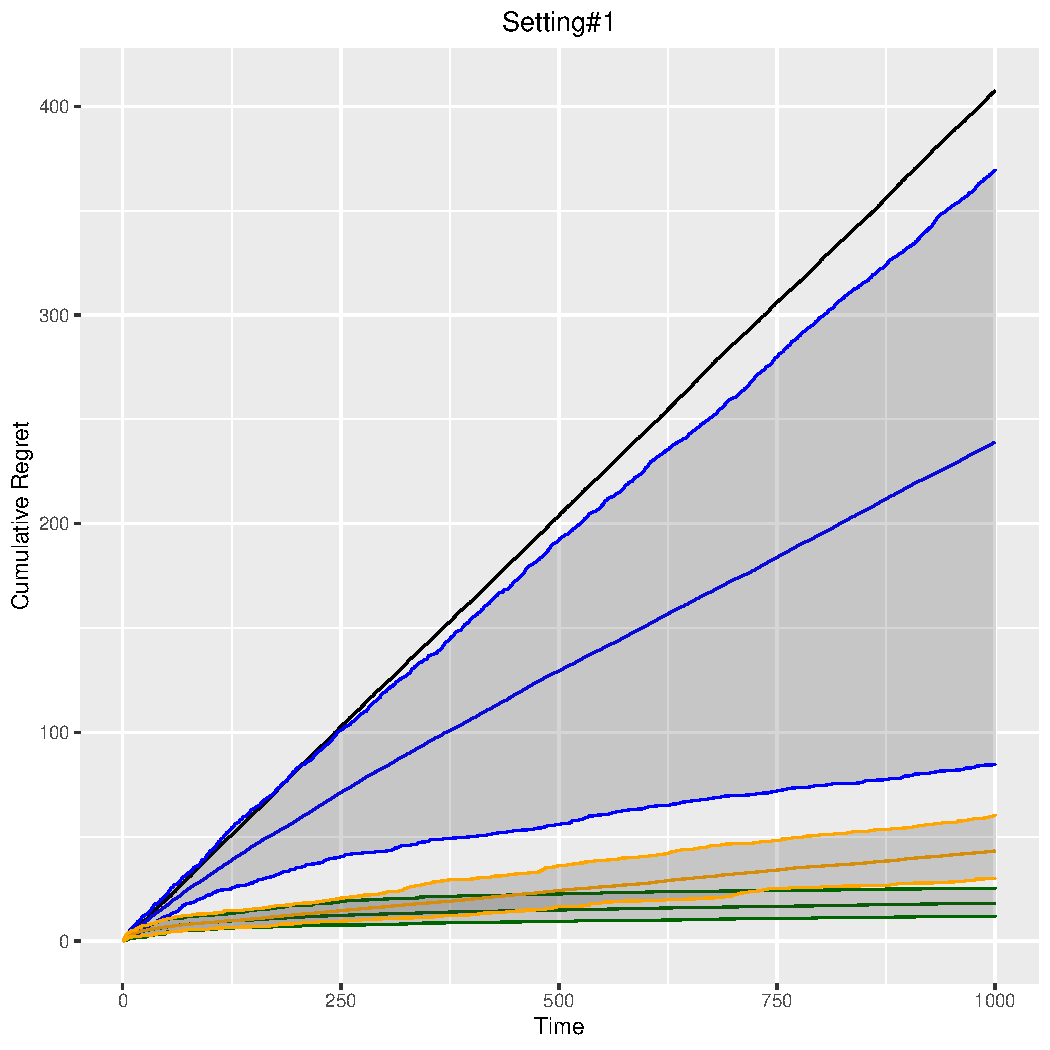
\includegraphics[scale = .4]{../../figures/experiment1-plot.pdf} &
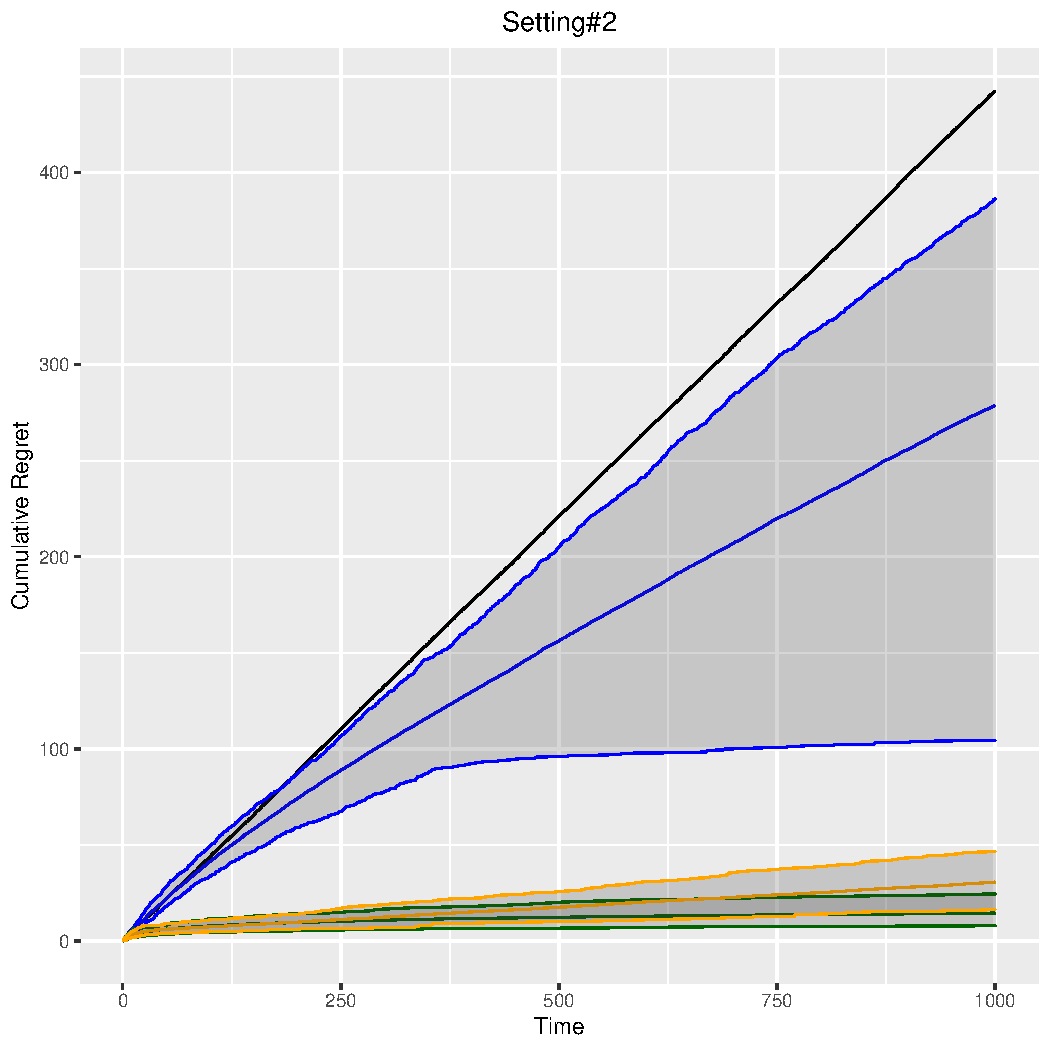
\includegraphics[scale = .4]{../../figures/experiment3-plot.pdf}
\end{tabular}
\caption{The average cumulative regret with the 5\% and 95\% percentile bands for
the MAB Thompson sampler and PG-TS with and without a rolling window for $M = 25$.
Both settings use $p = 6$ total context features with $K = 10$ and $K = 100$ arms.}
\label{figure:main-results}
\end{figure}

\section{Conclusion} \label{sec:conclusion}

The need for adaptive exploration of online retail continues to grow.  
While many have addressed this issue with multi-arm bandit algorithms with great
success, there is still room for improvement over simply estimating marginal
success rates.
Here we have explored a recent contextual extension of the well known Thompson
sampler, called P\'olya-Gamma Thompson Sampling, and empirically illustrated the 
potential gains in terms of minimizing the regret of the recommendations.
While improvements to the regret are realized, it does come at the cost of more
computation.
These computations can be somewhat mitigated by the rolling window we imposed.
Alternatively, computation could be reduced by computing updates in batches, 
rather than each iteration, or assuming the posterior covariance of the regression
coefficients to be diagonal, simplifying the inverse operation.
Regardless, as computational platforms continue to illustrate low-cost scalability,
the improvement to the recommendation platform seems deserving of consideration
for production systems.

\bibliography{cites.bib}
\bibliographystyle{apacite}

\end{document}